% Created by tikzDevice version 0.12.3.1 on 2022-09-01 15:55:47
% !TEX encoding = UTF-8 Unicode
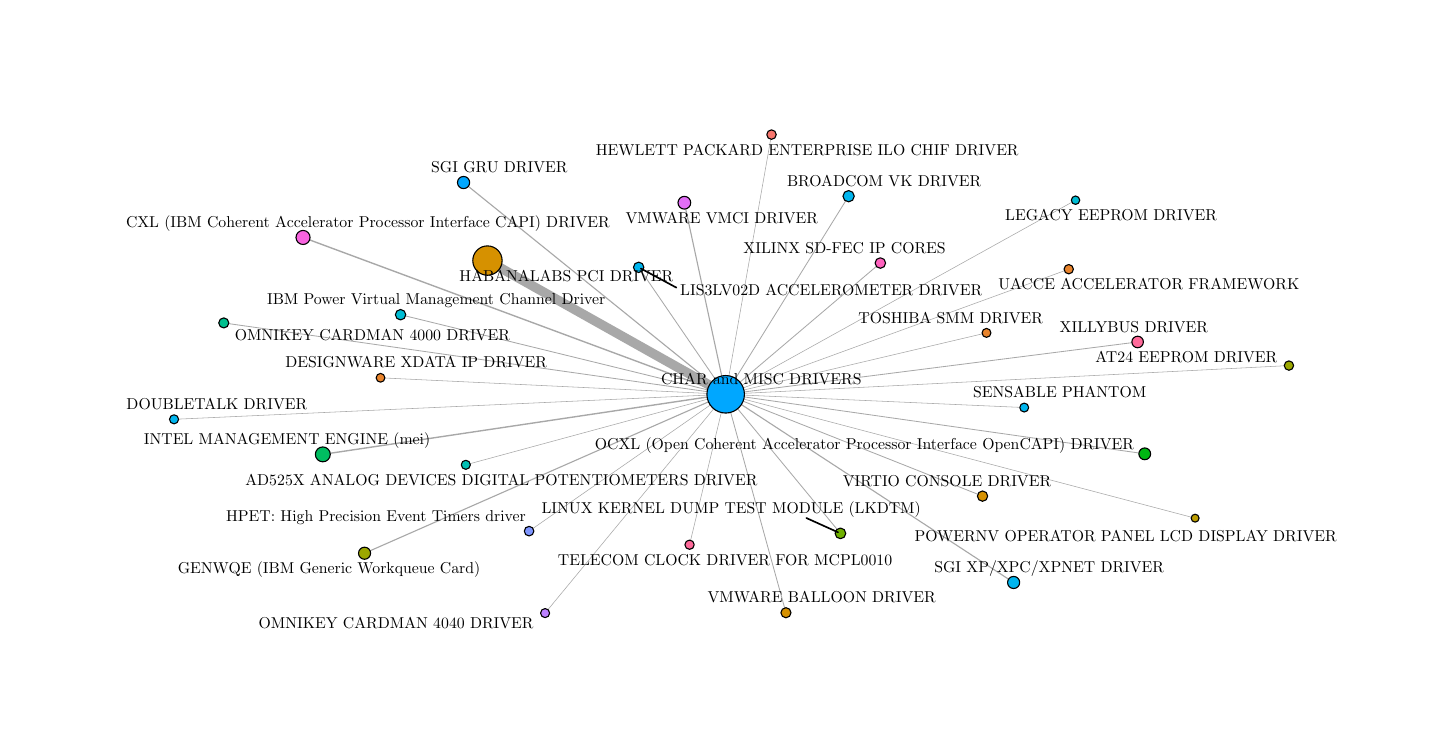
\begin{tikzpicture}[x=1pt,y=1pt]
\definecolor{fillColor}{RGB}{255,255,255}
\path[use as bounding box,fill=fillColor,fill opacity=0.00] (0,0) rectangle (505.89,252.94);
\begin{scope}
\path[clip] (  0.00,  0.00) rectangle (505.89,252.94);
\definecolor{fillColor}{RGB}{255,255,255}

\path[fill=fillColor] (  0.00,  0.00) rectangle (505.89,252.94);
\end{scope}
\begin{scope}
\path[clip] ( 32.75, 32.75) rectangle (475.89,222.94);
\definecolor{drawColor}{gray}{0.66}

\path[draw=drawColor,line width= 0.2pt,line join=round] (158.32, 94.98) -- (252.22,120.46);

\path[draw=drawColor,line width= 0.2pt,line join=round] (455.75,130.84) -- (252.22,120.46);

\path[draw=drawColor,line width= 0.3pt,line join=round] (296.64,192.04) -- (252.22,120.46);

\path[draw=drawColor,line width= 0.5pt,line join=round] (252.22,120.46) -- ( 99.50,177.13);

\path[draw=drawColor,line width= 0.2pt,line join=round] (252.22,120.46) -- (127.50,126.42);

\path[draw=drawColor,line width= 0.2pt,line join=round] (252.22,120.46) -- ( 52.89,111.42);

\path[draw=drawColor,line width= 0.4pt,line join=round] (252.22,120.46) -- (121.73, 63.03);

\path[draw=drawColor,line width= 3.4pt,line join=round] (252.22,120.46) -- (166.14,168.78);

\path[draw=drawColor,line width= 0.2pt,line join=round] (252.22,120.46) -- (268.78,214.30);

\path[draw=drawColor,line width= 0.2pt,line join=round] (252.22,120.46) -- (181.18, 71.01);

\path[draw=drawColor,line width= 0.3pt,line join=round] (252.22,120.46) -- (134.74,149.22);

\path[draw=drawColor,line width= 0.5pt,line join=round] (252.22,120.46) -- (106.65, 98.75);

\path[draw=drawColor,line width= 0.2pt,line join=round] (252.22,120.46) -- (378.64,190.59);

\path[draw=drawColor,line width= 0.3pt,line join=round] (252.22,120.46) -- (293.69, 70.20);

\path[draw=drawColor,line width= 0.3pt,line join=round] (252.22,120.46) -- (220.78,166.34);

\path[draw=drawColor,line width= 0.3pt,line join=round] (252.22,120.46) -- (403.65, 98.95);

\path[draw=drawColor,line width= 0.3pt,line join=round] (252.22,120.46) -- ( 70.86,146.25);

\path[draw=drawColor,line width= 0.2pt,line join=round] (252.22,120.46) -- (186.97, 41.40);

\path[draw=drawColor,line width= 0.2pt,line join=round] (252.22,120.46) -- (421.85, 75.70);

\path[draw=drawColor,line width= 0.2pt,line join=round] (252.22,120.46) -- (360.10,115.67);

\path[draw=drawColor,line width= 0.4pt,line join=round] (252.22,120.46) -- (157.51,196.98);

\path[draw=drawColor,line width= 0.4pt,line join=round] (252.22,120.46) -- (356.27, 52.46);

\path[draw=drawColor,line width= 0.2pt,line join=round] (252.22,120.46) -- (239.17, 66.10);

\path[draw=drawColor,line width= 0.2pt,line join=round] (252.22,120.46) -- (346.47,142.65);

\path[draw=drawColor,line width= 0.2pt,line join=round] (252.22,120.46) -- (376.18,165.66);

\path[draw=drawColor,line width= 0.3pt,line join=round] (252.22,120.46) -- (345.04, 83.66);

\path[draw=drawColor,line width= 0.3pt,line join=round] (252.22,120.46) -- (274.00, 41.53);

\path[draw=drawColor,line width= 0.4pt,line join=round] (252.22,120.46) -- (237.29,189.68);

\path[draw=drawColor,line width= 0.3pt,line join=round] (252.22,120.46) -- (308.11,167.89);

\path[draw=drawColor,line width= 0.3pt,line join=round] (252.22,120.46) -- (401.08,139.37);
\definecolor{drawColor}{RGB}{0,0,0}
\definecolor{fillColor}{RGB}{0,192,180}

\path[draw=drawColor,line width= 0.4pt,line join=round,line cap=round,fill=fillColor] (158.32, 94.98) circle (  1.64);
\definecolor{fillColor}{RGB}{156,167,0}

\path[draw=drawColor,line width= 0.4pt,line join=round,line cap=round,fill=fillColor] (455.75,130.84) circle (  1.69);
\definecolor{fillColor}{RGB}{0,181,238}

\path[draw=drawColor,line width= 0.4pt,line join=round,line cap=round,fill=fillColor] (296.64,192.04) circle (  2.04);
\definecolor{fillColor}{RGB}{0,167,255}

\path[draw=drawColor,line width= 0.4pt,line join=round,line cap=round,fill=fillColor] (252.22,120.46) circle (  6.78);
\definecolor{fillColor}{RGB}{248,99,223}

\path[draw=drawColor,line width= 0.4pt,line join=round,line cap=round,fill=fillColor] ( 99.50,177.13) circle (  2.54);
\definecolor{fillColor}{RGB}{233,132,44}

\path[draw=drawColor,line width= 0.4pt,line join=round,line cap=round,fill=fillColor] (127.50,126.42) circle (  1.58);
\definecolor{fillColor}{RGB}{0,181,238}

\path[draw=drawColor,line width= 0.4pt,line join=round,line cap=round,fill=fillColor] ( 52.89,111.42) circle (  1.64);
\definecolor{fillColor}{RGB}{156,167,0}

\path[draw=drawColor,line width= 0.4pt,line join=round,line cap=round,fill=fillColor] (121.73, 63.03) circle (  2.18);
\definecolor{fillColor}{RGB}{214,145,0}

\path[draw=drawColor,line width= 0.4pt,line join=round,line cap=round,fill=fillColor] (166.14,168.78) circle (  5.30);
\definecolor{fillColor}{RGB}{248,118,109}

\path[draw=drawColor,line width= 0.4pt,line join=round,line cap=round,fill=fillColor] (268.78,214.30) circle (  1.71);
\definecolor{fillColor}{RGB}{127,150,255}

\path[draw=drawColor,line width= 0.4pt,line join=round,line cap=round,fill=fillColor] (181.18, 71.01) circle (  1.73);
\definecolor{fillColor}{RGB}{0,189,212}

\path[draw=drawColor,line width= 0.4pt,line join=round,line cap=round,fill=fillColor] (134.74,149.22) circle (  1.88);
\definecolor{fillColor}{RGB}{0,189,97}

\path[draw=drawColor,line width= 0.4pt,line join=round,line cap=round,fill=fillColor] (106.65, 98.75) circle (  2.69);
\definecolor{fillColor}{RGB}{0,189,212}

\path[draw=drawColor,line width= 0.4pt,line join=round,line cap=round,fill=fillColor] (378.64,190.59) circle (  1.52);
\definecolor{fillColor}{RGB}{111,176,0}

\path[draw=drawColor,line width= 0.4pt,line join=round,line cap=round,fill=fillColor] (293.69, 70.20) circle (  1.93);
\definecolor{fillColor}{RGB}{0,181,238}

\path[draw=drawColor,line width= 0.4pt,line join=round,line cap=round,fill=fillColor] (220.78,166.34) circle (  1.88);
\definecolor{fillColor}{RGB}{0,184,19}

\path[draw=drawColor,line width= 0.4pt,line join=round,line cap=round,fill=fillColor] (403.65, 98.95) circle (  2.13);
\definecolor{fillColor}{RGB}{0,192,142}

\path[draw=drawColor,line width= 0.4pt,line join=round,line cap=round,fill=fillColor] ( 70.86,146.25) circle (  1.82);
\definecolor{fillColor}{RGB}{188,129,255}

\path[draw=drawColor,line width= 0.4pt,line join=round,line cap=round,fill=fillColor] (186.97, 41.40) circle (  1.64);
\definecolor{fillColor}{RGB}{188,157,0}

\path[draw=drawColor,line width= 0.4pt,line join=round,line cap=round,fill=fillColor] (421.85, 75.70) circle (  1.43);
\definecolor{fillColor}{RGB}{0,181,238}

\path[draw=drawColor,line width= 0.4pt,line join=round,line cap=round,fill=fillColor] (360.10,115.67) circle (  1.61);
\definecolor{fillColor}{RGB}{0,167,255}

\path[draw=drawColor,line width= 0.4pt,line join=round,line cap=round,fill=fillColor] (157.51,196.98) circle (  2.20);
\definecolor{fillColor}{RGB}{0,181,238}

\path[draw=drawColor,line width= 0.4pt,line join=round,line cap=round,fill=fillColor] (356.27, 52.46) circle (  2.19);
\definecolor{fillColor}{RGB}{255,106,154}

\path[draw=drawColor,line width= 0.4pt,line join=round,line cap=round,fill=fillColor] (239.17, 66.10) circle (  1.68);
\definecolor{fillColor}{RGB}{233,132,44}

\path[draw=drawColor,line width= 0.4pt,line join=round,line cap=round,fill=fillColor] (346.47,142.65) circle (  1.61);

\path[draw=drawColor,line width= 0.4pt,line join=round,line cap=round,fill=fillColor] (376.18,165.66) circle (  1.69);
\definecolor{fillColor}{RGB}{214,145,0}

\path[draw=drawColor,line width= 0.4pt,line join=round,line cap=round,fill=fillColor] (345.04, 83.66) circle (  1.86);

\path[draw=drawColor,line width= 0.4pt,line join=round,line cap=round,fill=fillColor] (274.00, 41.53) circle (  1.82);
\definecolor{fillColor}{RGB}{226,110,247}

\path[draw=drawColor,line width= 0.4pt,line join=round,line cap=round,fill=fillColor] (237.29,189.68) circle (  2.30);
\definecolor{fillColor}{RGB}{255,98,191}

\path[draw=drawColor,line width= 0.4pt,line join=round,line cap=round,fill=fillColor] (308.11,167.89) circle (  1.90);
\definecolor{fillColor}{RGB}{255,106,154}

\path[draw=drawColor,line width= 0.4pt,line join=round,line cap=round,fill=fillColor] (401.08,139.37) circle (  2.08);

\path[draw=drawColor,line width= 0.6pt,line join=round,line cap=round] (281.37, 75.76) -- (292.82, 70.59);

\path[draw=drawColor,line width= 0.6pt,line join=round,line cap=round] (234.40,159.01) -- (221.57,165.91);

\node[text=drawColor,anchor=base,inner sep=0pt, outer sep=0pt, scale=  0.57] at (171.17, 87.50) {AD525X ANALOG DEVICES DIGITAL POTENTIOMETERS DRIVER};

\node[text=drawColor,anchor=base,inner sep=0pt, outer sep=0pt, scale=  0.57] at (418.70,131.88) {AT24 EEPROM DRIVER};

\node[text=drawColor,anchor=base,inner sep=0pt, outer sep=0pt, scale=  0.57] at (309.50,195.61) {BROADCOM VK DRIVER};

\node[text=drawColor,anchor=base,inner sep=0pt, outer sep=0pt, scale=  0.57] at (265.09,124.03) {CHAR and MISC DRIVERS};

\node[text=drawColor,anchor=base,inner sep=0pt, outer sep=0pt, scale=  0.57] at (122.94,180.69) {CXL (IBM Coherent Accelerator Processor Interface CAPI) DRIVER};

\node[text=drawColor,anchor=base,inner sep=0pt, outer sep=0pt, scale=  0.57] at (140.38,130.00) {DESIGNWARE XDATA IP DRIVER};

\node[text=drawColor,anchor=base,inner sep=0pt, outer sep=0pt, scale=  0.57] at ( 68.36,114.98) {DOUBLETALK DRIVER};

\node[text=drawColor,anchor=base,inner sep=0pt, outer sep=0pt, scale=  0.57] at (108.90, 55.55) {GENWQE (IBM Generic Workqueue Card)};

\node[text=drawColor,anchor=base,inner sep=0pt, outer sep=0pt, scale=  0.57] at (194.66,161.31) {HABANALABS PCI DRIVER};

\node[text=drawColor,anchor=base,inner sep=0pt, outer sep=0pt, scale=  0.57] at (281.68,206.81) {HEWLETT PACKARD ENTERPRISE ILO CHIF DRIVER};

\node[text=drawColor,anchor=base,inner sep=0pt, outer sep=0pt, scale=  0.57] at (125.84, 74.56) {HPET:	High Precision Event Timers driver};

\node[text=drawColor,anchor=base,inner sep=0pt, outer sep=0pt, scale=  0.57] at (147.61,152.79) {IBM Power Virtual Management Channel Driver};

\node[text=drawColor,anchor=base,inner sep=0pt, outer sep=0pt, scale=  0.57] at ( 93.71,102.34) {INTEL MANAGEMENT ENGINE (mei)};

\node[text=drawColor,anchor=base,inner sep=0pt, outer sep=0pt, scale=  0.57] at (391.50,183.12) {LEGACY EEPROM DRIVER};

\node[text=drawColor,anchor=base,inner sep=0pt, outer sep=0pt, scale=  0.57] at (254.23, 77.27) {LINUX KERNEL DUMP TEST MODULE (LKDTM)};

\node[text=drawColor,anchor=base,inner sep=0pt, outer sep=0pt, scale=  0.57] at (290.35,156.18) {LIS3LV02D ACCELEROMETER DRIVER};

\node[text=drawColor,anchor=base,inner sep=0pt, outer sep=0pt, scale=  0.57] at (302.39,100.47) {OCXL (Open Coherent Accelerator Processor Interface OpenCAPI) DRIVER};

\node[text=drawColor,anchor=base,inner sep=0pt, outer sep=0pt, scale=  0.57] at (124.57,139.97) {OMNIKEY CARDMAN 4000 DRIVER};

\node[text=drawColor,anchor=base,inner sep=0pt, outer sep=0pt, scale=  0.57] at (133.13, 35.76) {OMNIKEY CARDMAN 4040 DRIVER};

\node[text=drawColor,anchor=base,inner sep=0pt, outer sep=0pt, scale=  0.57] at (396.74, 67.37) {POWERNV OPERATOR PANEL LCD DISPLAY DRIVER};

\node[text=drawColor,anchor=base,inner sep=0pt, outer sep=0pt, scale=  0.57] at (372.93,119.22) {SENSABLE PHANTOM};

\node[text=drawColor,anchor=base,inner sep=0pt, outer sep=0pt, scale=  0.57] at (170.43,200.58) {SGI GRU DRIVER};

\node[text=drawColor,anchor=base,inner sep=0pt, outer sep=0pt, scale=  0.57] at (369.13, 56.02) {SGI XP/XPC/XPNET DRIVER};

\node[text=drawColor,anchor=base,inner sep=0pt, outer sep=0pt, scale=  0.57] at (252.01, 58.63) {TELECOM CLOCK DRIVER FOR MCPL0010};

\node[text=drawColor,anchor=base,inner sep=0pt, outer sep=0pt, scale=  0.57] at (333.55,146.21) {TOSHIBA SMM DRIVER};

\node[text=drawColor,anchor=base,inner sep=0pt, outer sep=0pt, scale=  0.57] at (405.11,158.18) {UACCE ACCELERATOR FRAMEWORK};

\node[text=drawColor,anchor=base,inner sep=0pt, outer sep=0pt, scale=  0.57] at (332.19, 87.24) {VIRTIO CONSOLE DRIVER};

\node[text=drawColor,anchor=base,inner sep=0pt, outer sep=0pt, scale=  0.57] at (286.91, 45.09) {VMWARE BALLOON DRIVER};

\node[text=drawColor,anchor=base,inner sep=0pt, outer sep=0pt, scale=  0.57] at (250.81,182.17) {VMWARE VMCI DRIVER};

\node[text=drawColor,anchor=base,inner sep=0pt, outer sep=0pt, scale=  0.57] at (295.20,171.48) {XILINX SD-FEC IP CORES};

\node[text=drawColor,anchor=base,inner sep=0pt, outer sep=0pt, scale=  0.57] at (399.73,142.94) {XILLYBUS DRIVER};
\end{scope}
\end{tikzpicture}
